% Structure:
% - Introduction
% - Background
% - Problem
% -- Quadratics
% -- Cocyclics
% -- Monogenics
% -- General absolute
% - Applications to elliptics over Q
% - Conclusion


\documentclass[12pt,a4paper,abstracton,bibtotoc]{scrreprt}

\author{Alex J. Best \\ {\large Supervised by Dr. Lassina Demb\'el\'e}}
\date{2014}
\title{Finding orders with prescribed index in number fields}

\usepackage{amsmath, amssymb, amsfonts, amsthm, hyperref, listings, tikz, algorithm2e, graphicx, enumerate}
\usepackage[utf8]{inputenc}
\usepackage[T1]{fontenc}
\usepackage[english]{babel}
\usepackage{setspace}
\onehalfspacing

\theoremstyle{definition}
\newtheorem{thm}{Theorem}
\newtheorem{lem}{Lemma}
\newtheorem{cor}{Corollary}
\newtheorem{prop}{Proposition}
\newtheorem{defn}{Definition}
\newtheorem{defns}{Definitions}
\newtheorem{prob}{Problem}
\newtheorem{ex}{Example}
\newtheorem{rem}{Remark}
\newtheorem{nota}{Notation}
\newtheorem{alg}{Algorithm}

\setcounter{tocdepth}{3}

\lstset{
basicstyle=\footnotesize,       % the size of the fonts that are used for the code
showspaces=false,               % show spaces adding particular underscores
showstringspaces=false,         % underline spaces within strings
showtabs=false,                 % show tabs within strings adding particular underscores
frame=single,           % adds a frame around the code
captionpos=b,           % sets the caption-position to bottom
breaklines=true,        % sets automatic line breaking
breakatwhitespace=false,    % sets if automatic breaks should only happen at whitespace
}

\graphicspath{{img/}}

\newcommand{\QQ}{\mathbf{Q}}
\newcommand{\RR}{\mathbf{R}}
\newcommand{\CC}{\mathbf{C}}
\newcommand{\ZZ}{\mathbf{Z}}
\newcommand{\p}{\mathfrak{p}}
\newcommand{\q}{\mathfrak{q}}
\renewcommand{\O}{\mathcal{O}}

\DeclareMathOperator{\Orders}{Orders}
\DeclareMathOperator{\Ann}{Ann}
\DeclareMathOperator{\End}{End}
\DeclareMathOperator{\Mat}{Mat}
\DeclareMathOperator{\disc}{disc}
\DeclareMathOperator{\ord}{ord}
\DeclareMathOperator{\im}{im}
\DeclareMathOperator{\id}{id}

\begin{document}
\maketitle
\newpage\null\thispagestyle{empty}\newpage

\begin{abstract}
Orders of number fields are common objects of study in algebraic number theory.
Here we develop methods to obtain all orders with a specified index inside another given one.
The performance and coverage of these methods is discussed.
We also apply these techniques to a problem relating to elliptic curves over the rational numbers.

\smallskip
\noindent \textbf{Keywords.} Number theory, algebraic number theory, elliptic curves, number fields, algorithms.
\end{abstract}

\newpage\null\thispagestyle{empty}\newpage

\tableofcontents

\chapter{Introduction}
In this report we develop algorithmic methods for the solution of a problem arising from algebraic number theory.
Specifically we develop methods to find all orders of an algebraic number field with a given index inside another order.
We detail some situations in which these algorithms can be applied at the end.
Though the problem is a natural one we do not know of any previous work with exactly the same aim as ours.
Instead there is some existing work that relates to special cases of our problem, these are discussed in their relevant sections.

The report is organised as follows.
We first go through the background material needed to motivate, define and describe the solution of our problems in chapter~\ref{chap:background}.
In section~\ref{sec:ca} we cover some commutative algebra dealing with the basic properties of modules over rings, after this in section~\ref{sec:ant} we move into algebraic number theory defining the key notions needed to study orders and considering the reasons such ideas were introduced.
We finish up the background material in section~\ref{sec:ell} with an introduction to the theory of elliptic curves, which will be one of the areas we will apply our methods to.

Chapter~\ref{chap:prob} is where we consider our main problem and solutions to it.
First we define the problems themselves and discuss the interest in studying them.
After this in the rest of chapter~\ref{chap:prob} we detail the techniques used to solve the problems considered, starting with some special cases before moving onto more general results.
Next we discuss the advantages of the algorithms developed and ideas worth bearing in mind when implementing these algorithms.

Finally in chapter~\ref{chap:ellapp} we move on to looking at an interesting application of these methods to finding elliptic curves with given properties.


\chapter{Background material}
\label{chap:background}

In this section we fix several definitions and important results from algebraic number theory and commutative algebra.
We assume only fairly basic knowledge of abstract algebra, such as the notions of groups, rings and fields.

The results given here are well known and are used throughout the rest of the report.

\section{Commutative algebra}
\label{sec:ca}
We introduce several notions and results that will be useful to us throughout the report, proofs for those results not proved here can be found in many textbooks on commutative algebra, such as \cite{am} or \cite{matsumura}.

All rings here are commutative with an identity element.
\begin{defn}[Module]
Given a ring $R$ we define an \emph{$R$-module} $M$ to be an abelian group under addition, with a scalar multiplication map $\cdot \colon R\times M \to M$ satisfying
\begin{align*}
1\cdot m &= m \; &&\text{for all } m\in M \\
r_1\cdot(r_2 \cdot m) &= (r_1r_2)\cdot m \; &&\text{for all } r_1,r_2\in R,\; m\in M \\
r\cdot(m_1 + m_2) &= r\cdot m_1 + r\cdot m_2 \; &&\text{for all } r\in R, \; m_1,m_2\in M \\
(r_1 + r_2)\cdot m &= r_1\cdot m + r_2\cdot m \; &&\text{for all } r_1,r_2\in R, \; m_1\in M
\end{align*}
\end{defn}

We often refer to elements of the ring $R$ as \emph{scalars}.

From now on we will omit the notation $\cdot$ for scalar multiplication as it will be clear from context when the multiplication is taking place in the ring $R$ or on a module $M$.
We will also not make explicit the ring $R$ involved if it is not relevant to the discussion at hand, instead referring simply to a \emph{module}.

The most common modules we will use here will be $\ZZ$-modules such as:
\begin{ex}
\[
\ZZ,\ \{(a,b)\mid a,b\in \ZZ\},\text{ or }\{a\sqrt{2} + b\sqrt[3]{2}\mid a,b\in \ZZ\}.
\]
\end{ex}
In fact every abelian group can be given a $\ZZ$-module structure so of course they are ubiquitous in commutative algebra, nevertheless it is useful to think of the modules used here in terms of $\ZZ$ rather than as abstract abelian groups.
We now list some standard definitions that are used to talk about how different modules relate to one another and describe ways of constructing new modules from old.

\begin{defn}[Module homomorphism]
Given $R$-modules $M_1$ and $M_2$, a function $f\colon M_1 \to M_2$ satisfying
\begin{align*}
f(rm) &= rf(m) &&\text{ for all $r\in R$, $m\in M_1$}\\
f(m + m') &= f(m) + f(m')&&\text{ for all $m,m'\in M_1$}
\end{align*}
is called an \emph{$R$-module homomorphism} or simply a \emph{module homomorphism} when the ring is clear.
We also use the term map for this concept.
\end{defn}

\begin{defn}[Isomorphism of modules]
Two $R$-modules $M_1$ and $M_2$ are said to be \emph{isomorphic} is there exists a bijective module homomorphism between them. 
In this case we write $M_1\cong M_2$.
\end{defn}

Module isomorphism is an equivalence relation on the class of all modules and so we often think of two isomorphic modules as being the same, just written in a different manner.

\begin{defn}[Submodule]
A \emph{submodule} $N$ of a module $M$ is a module whose elements all belong to $M$ and whose operations are the same as those from $M$ on the elements on $N$.
\end{defn}

\begin{defn}[Quotient module]
The \emph{quotient module} of two $R$-modules $M$ and $N$ where $N$ is a submodule of $M$ is defined to be the $R$-module whose additive group quotient abelian group $M/N$ under addition with scalar multiplication given by
\[
r\cdot(m + N) = rm + N\text{ for all }r\in R,\ m\in M.
\]
This module is denoted by $M/N$.
\end{defn}

\begin{defn}[Index]
Given a module $N$ that is a submodule of a module $m$ the \emph{index} of $N$ in $M$, denoted $[M:N]$ is the size of the quotient module $M / N$.
\end{defn}

\begin{defn}[Direct sum]
Given two $R$-modules $M_1$ and $M_2$ we define their \emph{direct sum} (denoted $\oplus$) to be the module with element set $M_1 \times M_2$ and operations given by the operations of $M_1$ and $M_2$ performed elementwise. i.e.
\begin{align*}
r\cdot(m_1,m_2) &= (r\cdot m_1, r\cdot m_2)\\
(m_1,m_2) + (m_1',m_2') &= (m_1 + m_1',m_2+m_2').
\end{align*}
\end{defn}

Not that this is in general distinct from when we have $M_1$ and $M_2$ submodules of some module $N$ and write
\[
M_1 + M_2 = \{m_1 + m_2 \mid m_1\in M_1,\ m_2\in M_2\}.
\]
For example with this elementwise addition we have $M + M = M$ for any module $M$, whereas $M\oplus M$ is not isomorphic to $M$ unless $M$ is the trivial module (i.e. the module containing only a zero element and no others).

The well known isomorphism theorems also hold for modules, we will need all three.

\begin{thm}[First isomorphism theorem for modules]
Given a surjective module homomorphism $f\colon M \to N$ the kernel of $f$ is a submodule of $M$ and
\[
M/\ker(f) \cong N.
\]
\end{thm}

\begin{thm}[Second isomorphism theorem for modules]
Given a module $M$ with submodules $N_1$ and $N_2$ the sum $N_1 + N_2$ is a submodule of $M$ too, such that $N_1 \cap N_2$ is a submodule of $N_1$ and we have the isomorphism
\[
(N_1 + N_2)/N_2 \cong N_1/(N_1 \cap N_2).
\]
\end{thm}

\begin{thm}[Third isomorphism theorem for modules]
Given a chain of submodules $M_1 \subseteq M_2 \subseteq M_3$ the quotient module $M_2/M_1$ is a submodule of $M_3/M_1$ and we have an isomorphism
\[
(M_3/M_1)/(M_2/M_1) \cong (M_3/M_2).
\]
\end{thm}

An easy consequence of this relating the indices of submodules is worth noting.

\begin{cor}
\label{cor:indexmult}
Given a chain of submodules $M_1 \subseteq M_2 \subseteq M_3$ with finite indices inside each other we have
\[
[M_3:M_1] = [M_3:M_2][M_2:M_1].
\]
\end{cor}

\minisec{}
We now define a property of modules that makes them easier to work with and, importantly, easier to do computations with.

\begin{defn}[Finitely generated]
An $R$-module $M$ is \emph{finitely} generated if there is a \emph{finite} set $B\subset M$ such that any $m\in M$ can be written as
\[m = \sum_{b\in B} \alpha_b b\]
for some coefficients $\alpha_b \in R$.
\end{defn}

\begin{defn}[Torsion submodule]
The \emph{torsion submodule} $M_\text{tors}$ of an $R$-module $M$ is the set
\[
\{m\in M \mid \exists\; r \in R\setminus 0 \text{ such that } rm = 0\}.
\]
This is the set of elements that are killed by some non-zero scalar.
As implied by the name this is always submodule of $M$.
\end{defn}

A module $M$ is called a torsion module if $M_\text{tors} = M$, and torsion-free if $M_\text{tors} = 0$.

\begin{defn}[Rank of a $\ZZ$-module]
Given a $\ZZ$-module $M$ we can always write $M = M_\text{tors} \oplus \ZZ^r$ for some unique $r\in \ZZ_{\ge 0}$.
This $r$ is called the \emph{rank} of the $\ZZ$-module.
\end{defn}

This notion generalises in a natural way to modules over other principal ideal domains.

\begin{ex}
\[M = \ZZ^2 = \{(a,b)\mid a,b\in \ZZ\}\]
is a torsion free $\ZZ$ module. Let
\[N = \{(2c,0) \mid c\in\ZZ\} \cong \ZZ\]
be a submodule of $M$.
Then the quotient module
\[M/N \cong (\ZZ/2\ZZ)\times \ZZ\]
has torsion submodule $(M/N)_\text{tors}$ equal to $\ZZ/2\ZZ$ and is of rank 1.
\end{ex}

\begin{defn}[Short exact sequence]
A \emph{short exact sequence of $R$-modules} is a sequence of $R$-modules and maps between them, drawn as
\[
0 \to M_1 \xrightarrow{f_1} M_2 \xrightarrow{f_2} M_3 \to 0
\]
such that for every occurrence of a triple $N_1 \xrightarrow{g_1} N_2 \xrightarrow{g_2} N_3$ we have $\im(g_1) = \ker(g_2)$.
\end{defn}

In any short exact sequence we therefore have $f_1$ injective and $f_2$ surjective.

\begin{defn}[Split short exact sequence]
A short exact sequence $0 \to M_1 \xrightarrow{q} M_2 \xrightarrow{r} M_3 \to 0$ is called \emph{split} if any of the following equivalent conditions hold:
\begin{enumerate}[(i)]
\item There is a map $t\colon M_2 \to M_1$ such that $t\circ q$ is the identity on $M_1$.
\item There is a map $u\colon M_3 \to M_2$ such that $u\circ r$ is the identity on $M_2$.
\item $M_2 \cong M_1 \oplus M_3$.
\end{enumerate}
\end{defn}

We have one more notion to define.

\begin{defn}[$R$-algebra]
A ring $S$ with a ring homomorphism $f$ from another ring $R$ to $S$ is called an \emph{$R$-algebra}.
The homomorphism gives $S$ the structure of an $R$-module by letting $r\cdot s = f(r)s$.
\end{defn}

\section{Algebraic number theory}
\label{sec:ant}

Algebraic number began with the study of algebraic numbers and their uses in solving Diophantine equations.
The subject has since expanded to encompass a huge amount of mathematics involving the use of algebraic techniques to tackle number theoretic problems.
We give a short introduction to the results relevant to us here.
As above, more details about anything not proved here can be found in any of the many texts on algebraic number theory, for example \cite{neukirch}, \cite{lang}, \cite{narkiewicz} or \cite{stewtall}.

\begin{defn}[Number field]
A \emph{number field} $K$ is a field that is also a finite dimensional $\QQ$-vector space.
\end{defn}

\begin{ex}\label{ex:quad}
We write $\QQ(\sqrt{3})$ for the smallest field containing both $\QQ$ and $\sqrt{3}$, it is clear that the set
\[
\{a + b\sqrt{3}\mid a,b \in \QQ\}
\]
must be contained in such a field.
But we can also see that this set is closed under addition, subtraction, multiplication and non-zero division, and hence this set is the field $\QQ(\sqrt{3})$.

Here we see that $\QQ(\sqrt{3})$ has dimension 2 as a vector space over $\QQ$.
\end{ex}

\begin{defn}[Degree of a number field]
The dimension of a number field $K$ as a $\QQ$ vector space is called the \emph{degree} of $K$, denoted $[K:\QQ]$.

We say that number fields of degree 2, such as in example~\ref{ex:quad} above are \emph{quadratic}.
Similarly degree 3 number fields are called \emph{cubic}.
\end{defn}

\minisec{}
The following few definitions are central to the whole problem.

A number field will have a large quantity of subrings, only some of which are of real number theoretic interest.
So we distinguish some subrings that have desirable properties and single them out for study.

\begin{defn}[Order]
An \emph{order} of a number field $K$ is a subring of $K$ that is finitely generated as a $\ZZ$-module, and of rank equal to the degree of $K$ (this is the maximal rank).
\end{defn}

By definition orders have finite bases over $\ZZ$ and so we will often represent orders by writing them as sums 
\[
\O = \ZZ\alpha_1 + \ZZ \alpha_2 + \cdots + \ZZ \alpha_n.
\]
We also use the notation $\ZZ[\alpha]$ to mean the ring of polynomials expressions in $\alpha$ with integer coefficients, provided $\alpha$ is an algebraic integer this will be an order.

\begin{defn}[Ring of integers]
The \emph{ring of integers}, denoted $\ZZ_K$, of a number field $K$ is the unique maximal order.
\end{defn}

The terminology for this ring comes from the fact that its behaviour is analogous to the way $\ZZ$ behaves inside $\QQ$.
As we will see later the maximal order of a quadratic number field is easy to determine but the complexity of such calculations increases with the degree.

The notion of index introduced earlier applies here and as all orders lie inside the ring of integers we can always find the index of an order $\O$ inside $\ZZ_K$.
If we just use the term index of an order, without specifying another containing it, we will mean exactly this, the index inside the maximal order.

\begin{ex}
\[
[\ZZ\cdot 1 + \ZZ\cdot \sqrt{2} : \ZZ \cdot 1 + \ZZ \cdot 2\sqrt{2}] = 2.
\]
\end{ex}

In figure~\ref{fig:sageord} one embedding into the complex plane of the ring of integers of $\QQ[x]/(x^2 + 19)\cong \QQ(\sqrt{-19})$ is shown.
Highlighted in bold is a suborder of index 3 in this order.
\begin{figure}
\centering
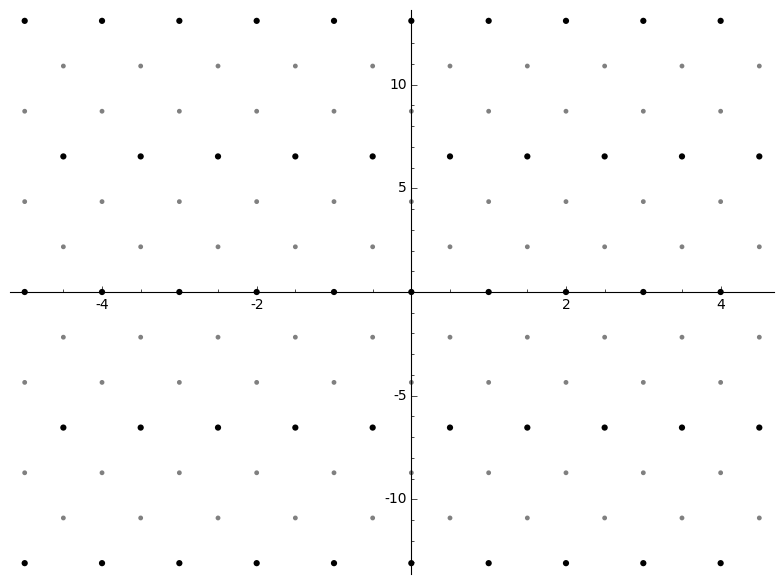
\includegraphics[scale=0.6]{sageord}
\caption{\label{fig:sageord} An embedding in $\CC$ of the ring of integers of $\QQ(\sqrt{-19})$ and an index 3 suborder.}
\end{figure}

%P.<x> = QQ[]
%K = NumberField(x^2 + 19, 'a')
%ZK = K.maximal_order()
%OK = K.order(3*ZK.0)
%print ZK.basis()
%f = K.embeddings(CC)[0]
%pts = []
%pts2 = []
%for x in range(-10,10):
%    for y in range(-10,10):
%        if f(x*ZK.0 + y*ZK.1).imag().abs() < 15: 
%            pts.append(f(x*ZK.0 + y*ZK.1))
%        if f(x*OK.0 + y*OK.1).imag().abs() < 15: 
%            pts2.append(f(x*OK.0 + y*OK.1))
%
%list_plot(pts,color="gray",size=12) + list_plot(pts2,color="black",size=20)


\section{Elliptic curves}
\label{sec:ell}

We now introduce the background material relevant to elliptic curves, one of the intended applications of these methods.
This is not required for the main problem discussed in chapter~\ref{chap:prob}, but chapter~\ref{chap:ellapp} uses these ideas heavily.
As with the above sections everything here can be found in textbooks on elliptic curves (such as \cite{knapp} or \cite{cassels}), we offer a rapid summary, moving quickly to the notions relevant to this project.

\begin{defn}[Elliptic curve]
For us an \emph{elliptic curve} $E$ defined over a field $K$ will be given by a binary cubic equation of the form
\[
y^2 + a_1xy + a_3y = x^3 + a_2x^2 + a_4x + a_6\text{ with }a_i\in K.
\]
To such a curve we assign several $b$ invariants based on the coefficients in the definition as follows
\begin{align*}
b_2 &= a_1^2 + 4a_2,\\
b_4 &= 2a_4 + a_1a_3,\\
b_6 &= a_3^2 + 4a_6,\\
b_8 &= a_1^2a_6 + 4a_2a_6 - a_1a_3a_4 + a_2a_3^2 -a_4^2.
\end{align*}
We then also require that the \emph{discriminant} $\Delta$ of $E$, given by
\[
\Delta = -b_2^2b_8 -8b_4^3 -27b_6^2 +9b_2b_4b_6,
\]
is not zero for $E$ to really be an elliptic curve.

Given an elliptic curve $E$ defined over a field $K$ with $K \subset K'$ another field, we let $E(K')$ be the set of points in $K'\times K'$ satisfying the equation defining $E$, along with an extra point $\infty$.
This additional point is called the point at infinity, the reasons for its inclusion in the set should become clear later.
\end{defn}

The condition on $\Delta$ given above is to ensure that our curve does not have any points where both the derivatives with respect to $x$ and $y$ vanish, such a point is called a singular point and the existence of such a point causes the behaviour of the curve to differ highly from what we would normally expect.

\begin{ex}
Let 
\[
E \colon y^2 + 2xy + y = x^3 - 2x + 3
\]
be an elliptic curve.
Then we can see that $(1,(\sqrt{17}-3)/2)\in E(\RR) \subset E(\CC)$ as the coordinates satisfy the equation defining the curve.

We can plot the real points of this curve, such a plot is shown in figure~\ref{fig:ec}.
This plot of the real points is typical for an elliptic curve, though there can easily be two connected components rather than one as in this case.
\begin{figure}
\centering
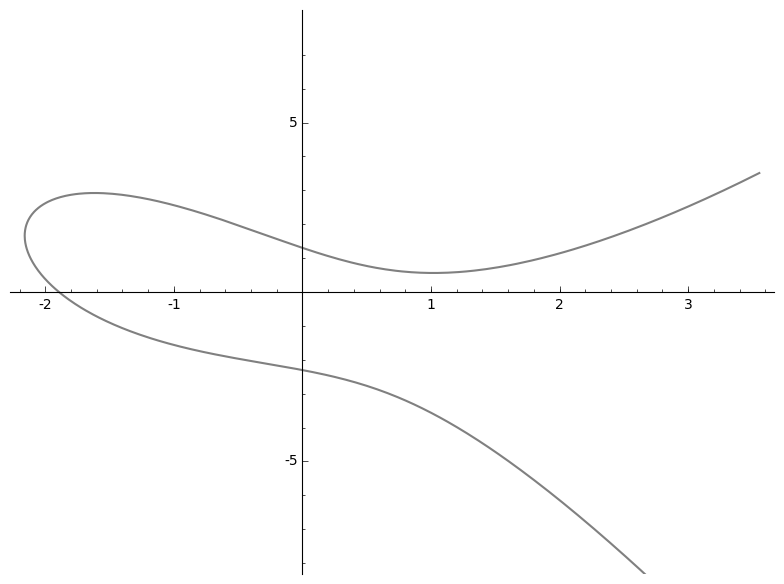
\includegraphics[scale=0.6]{sageec}
\caption{\label{fig:ec}The real points of $E \colon y^2 + 2xy + y = x^3 - 2x + 3$.}
\end{figure}
\end{ex}

One of the things that makes elliptic curves so interesting to study is the fact that we can define a natural way of adding points of the curve over some field, with this definition the set of points on the curve becomes a group.

\begin{defn}[Group law]
We define the sum of two points $P,Q\in E(K)$ for some field $K$ as follows, let $L$ be the line joining $P$ and $Q$ (take $L$ to be the tangent at $P$ if $P=Q$).
Then $L$ intersects $E$ in three points (with multiplicity) so there is one point in addition to $P$ and $Q$ on both $L$ and $E$, call this point $R$.
Now there is at most one other point with the same $x$ coordinate as $R$ that lies on $E$, this is our sum $P+Q$.

In the above definition we think of the point at infinity as lying infinitely far away in the positive $y$ direction, therefore a line from $\infty$ to the point $P$ is the line through $P$ perpendicular to the $x$-axis.
\end{defn}

With this definition of addition the set of points of $E$ over some field $K$ is a group, and moreover this group is abelian (as the line through $P$ and $Q$ is the same as the line through $Q$ and $P$).
The identity element of our group is the point at infinity referred to above.
From now on we will denote the point $\infty\in E(K)$ as $0$, but still refer to it as \emph{at infinity}.

We want to consider some special maps between elliptic curves that respect both the curve and group structure.
\begin{defn}[Homomorphism of elliptic curves]
Let $E$ be an elliptic curve defined over a field $K$.
A group homomorphism $f\colon E \to E'$ such that there are polynomials $a,b,c,d\in \overline{K}[x,y]$ with
\[
f(x,y) = \left(\frac{a(x,y)}{b(x,y)},\frac{c(x,y)}{d(x,y)}\right) \text{ for } (x,y) \in E\setminus 0
\]
is called a \emph{homomorphism of elliptic curves}.
\end{defn}

\begin{defn}[Isomorphism of elliptic curves]
If we have two elliptic curves $E$ and $E'$ such that there exists homomorphisms $f\colon E \to E'$ and $g\colon E'\to E$ with $f\circ g = \id_{E'}$ and $g\circ f = \id_{E}$ then $E$ and $E'$ are called \emph{isomorphic}.
A homomorphism $f$ with an inverse $g$ as in the definition above is called an \emph{isomorphism}.
\end{defn}

We can also consider homomorphisms from a given elliptic curve to itself, these are known as \emph{endomorphisms} and they form a ring.

\begin{defn}[Endomorphism ring]
The \emph{endomorphism ring} of an elliptic curve is the set
\[
\End(E) = \{f\colon E \to E\mid f \text{ is a homomorphism of elliptic curves}\}
\]
with a ring structure given by $(f+g)(P) = f(P) + g(P)$ and multiplication is composition.
\end{defn}

As remarked above any abelian group can be regarded as a $\ZZ$-module $M$ in a natural way by letting 
\[n\cdot z = \underbrace{z + z + \cdots + z}_\text{$n$ times},\text{ for } n\in\ZZ_{\ge 0},\ z\in M\]
and letting $n\cdot z = (-n)\cdot(-z)$ for negative $n\in \ZZ$.
With this idea in mind $E(K)_\text{tors}$ is the set of points of $E$ defined over $K$ that can be added to themselves some finite number of times to get the point at infinity.
This is often called the \emph{torsion subgroup} of $E$.
It turns out that when $K = \QQ$ there are only a finite number of groups that $E(\QQ)_\text{tors}$ can be.

\begin{thm}[Mazur's torsion theorem]
\label{thm:tors}
Given an elliptic curve $E$ defined over the rationals $E(\QQ)_\text{tors}$ is one of:
\[
\ZZ/i\ZZ,\text{ for } i \in\{1,2,\ldots,9,10,12\}\text{ or }
\ZZ/2\ZZ \times \ZZ/2i\ZZ,\text{ for } i \in\{1,2,3,4\}.
\]
\end{thm}

In fact similar results have been obtained for quadratic fields too, for more detail on what is known about the torsion subgroup of an elliptic curve over a number field see \cite{sutherland}.

Sometimes it is necessary to talk about smaller subgroups of this group whose elements have order dividing some fixed $n$ and so we introduce the following definition.
\begin{defn}[$n$-division points]
For some $n\in\ZZ$ the set of \emph{$n$-division points} (or \emph{$n$-torsion points}) of $E$ over $K$ is
\[
E(K)[n] = \{P\in E(K) \mid nP = 0\}.
\]
The notation $E[n]$ then refers to $E(\overline{K})[n]$.
\end{defn}

\minisec{}
We are now ready to state in precise terms the problem we aimed to solve and to detail the methods used in its solution.


\chapter{Finding orders with prescribed index}
\label{chap:prob}

The aim of the project was to find a general method to solve the following problem, and moreover to find efficient algorithms that can solve the problem on any given inputs.

\begin{prob}
Given an order $R$ of an absolute number field $K$ and an integer $I$ find the set
\[
\Orders(R,I) = \left\{ \O\subseteq R \mid \O\text{ is a suborder},\ [R:\O] = I\right\}.
\]
\end{prob}

To find a suborder we really mean to compute a $\ZZ$ basis for the suborder in terms of the basis of the larger order.
Such a basis defines an order completely.

\minisec{}
One very natural extension of the above problem is to consider relative extensions of number fields.
More precisely we can generalise the above problem to the following one.

\begin{prob}
\label{prob:rel}
Given an extension of number fields $L|K$, a $\ZZ_K$-order $R$ of $L$ and an integer $I$ find the set
\[
\left\{ \O\subseteq R \mid \O\text{ is a $\ZZ_K$-suborder},\ [R:\O] = I\right\}.
\]
\end{prob}
Much of what follows should be extendible to relative orders fairly easily, however we do not consider this problem any further.

\minisec{}
We have defined our problem in terms of a general starting order and attempt to work with this hypothesis throughout.
However it is worth noting that as any order of a number field $K$ is contained in the maximal order $\ZZ_K$ we have that
\[
\Orders(R,I) = \Orders(\ZZ_K, I[\ZZ_K : R]) \cap \{\O\mid \O \text{ is a suborder of } R\}.
\]
So we can always reduce to the case where our base order is $\ZZ_K$ and filter out resulting orders not contained in $R$.
We try to avoid this algorithmically undesirable solution wherever possible though.

We now detail some methods to solve the problem in the absolute setting in varying generality.

\section{Quadratic number fields}

Quadratic number fields are the simplest non-trivial number fields and they have a large amount of structure which can often make them easier to work with than more general number fields.
As we will see, in this case the solution of our problem is very simple.

It is well known \cite{lang} that the ring of integers of a quadratic field $K = \QQ(\sqrt{d})$ for $d$ non-square always takes the form
\[\ZZ_K = \ZZ + \ZZ\alpha,\text{ with } \alpha =\begin{cases}
\sqrt{d}&\text{ if $d\equiv 2,3\pmod{4}$},\\
\frac{1+\sqrt{d}}{2}&\text{ if $d\equiv 1\pmod{4}$}.
\end{cases}\]

Indeed there is so little room for manoeuvre here that the following result on the structure of an order holds in this case.

\begin{prop}
\label{prop:quadord}
Every order $\O$ of a quadratic number field can be expressed as
\[
\O = \ZZ + \ZZ f\alpha
\]
for some $f\in \ZZ$, $\alpha$ as above.
\end{prop}

For a proof see \cite[pp. 133--134]{cox}.

\begin{defn}
The $f$ appearing in the above proposition is called the \emph{conductor} of the order $\O$.
Later we shall abuse this definition slightly by redefining the conductor to generalise this concept.
\end{defn}

Now it is clear that
\[
[\ZZ + \ZZ\alpha : \ZZ + \ZZ f \alpha] = |\ZZ/f\ZZ| = |f|.
\]
So we have an incredibly simple solution for quadratic number fields, there is exactly one order of a given index in $\ZZ_K$.
Hence in the quadratic case can say the following.

\begin{prop}
If $\ZZ_K = \ZZ + \ZZ\alpha$ and $R = \ZZ + \ZZ m\alpha$ then
\[
\Orders(R, I) = \{\ZZ + \ZZ Im\alpha\}.
\]
\end{prop}
\begin{proof}
This follows immediately from the above description of orders of $K$ (proposition~\ref{prop:quadord}) and the fact that the index is multiplicative (corollary \ref{cor:indexmult}).
\end{proof}

Orders in quadratic fields appear in the theory of elliptic curves with complex multiplication.
The endomorphism ring of an elliptic curve is either isomorphic to $\ZZ$ or an order $\O$ of an imaginary quadratic number field (i.e. a quadratic number field $K$ where $K\cap \RR \ne K$).
In the second case the curve is said to have \emph{complex multiplication}.
The theory of such curves is interesting and has practical applications in the field of cryptography and other areas, see \cite{schertz}.
A general solution to our problem is of course not particularly useful here as the situation is so simple.
However it is maybe conceivable that our methods could find application in generalisations of the theory of complex multiplication (to higher dimensional abelian varieties).
This is not a direction we have pursued but it might be worthwhile to do so.

\section{Monogenic orders}
\label{sec:monogenic}
We now look at a special class of orders that have been studied extensively by other authors, though the focus of their methods has been slightly different to ours.

\begin{defn}[Monogenic order]
An order of the form $\ZZ[\alpha]$ for some algebraic integer $\alpha$ is called \emph{monogenic}.
\end{defn}

Monogenic orders can be easier to work with than more general orders and are common in algebraic number theory.
The ease of computing with them comes from the fact that
\[
\ZZ[\alpha] = \ZZ + \ZZ\alpha + \ZZ\alpha^2 + \cdots + \ZZ\alpha^{n-1}
\]
and so $\{1,\alpha,\ldots,\alpha^{n-1}\}$ is a basis for $\ZZ[\alpha]$ as a $\ZZ$ module (here $n$ is $[K : \QQ]$).
With this basis computing products of elements with a computer (and by hand) is simpler to do than in general making them natural bases to work with.
A basis of this form is known as a \emph{power basis}.

\minisec{}
Several authors have studied the problem of finding monogenic orders, mostly with a view to showing that the ring of integers is monogenic and finding elements $\alpha$ such that $\ZZ_K = \ZZ[\alpha]$ in this case.
This is essentially the problem of finding monogenic orders of index 1 in $\ZZ_K$.
An up-to-date account of the methods known for performing such computations is given in Istv\'an Ga\'al's book \cite{gaal}.
Here we attempt to convey the approach these methods take without going into detail concerning the exact methods of solution.

Given an order $\O$ of a number field $K$ of degree $n$ such that
\[
\O = \ZZ + \ZZ\omega_2 + \cdots + \ZZ\omega_n.
\]
We can calculate the index of the order $\ZZ[\alpha]$ where $\alpha = x_1 + x_2\omega_2 + \cdots x_n\omega_n\in \O$ as follows.

First we recall \cite[pp. 11--15]{neukirch} that the discriminant of an order $\O$ in a number field $K$ is given by
\[
d(\O) = \det(\sigma_i(\alpha_j))^2
\]
where the $\sigma_i$ are the embeddings of $K$ into $\CC$ and the $\alpha_j$ are a $\ZZ$-basis for $\O$.
Now given two orders $\O \subset \O'$ it is the case that
\[
d(\O) = [\O':\O]^2 d(\O')
\]
And so the index is given by
\begin{equation}
[\O':\O] = \sqrt{\frac{d(\O)}{d(\O')}}.
\label{eq:indexsq}
\end{equation}
In the special case where $\O = \ZZ[\alpha]$ a $\ZZ$-basis for $\O$ is $1,\alpha,\ldots,\alpha^{n-1}$ and we have that
\begin{align*}
d(\O) &= \det\begin{pmatrix}
1 & \alpha & \cdots & \alpha^{n-1}\\
1 & \sigma_1(\alpha) & \cdots & \sigma_1(\alpha)^{n-1}\\
\vdots & \vdots & \ddots & \vdots\\
1 & \sigma_{n-1}(\alpha) & \cdots & \sigma_{n-1}(\alpha)^{n-1}
\end{pmatrix}^2\\
&=\prod_{1\le i<j\le n} (\sigma_i(\alpha) - \sigma_j(\alpha))^2
\end{align*}

Now if we take $\alpha$ to be given by $\alpha = x_1 + x_2\omega_2 + \cdots x_n\omega_n$ we have that in fact
\[
\prod_{1\le i<j\le n} (\sigma_i(\alpha) - \sigma_j(\alpha))^2 = \prod_{1\le i<j\le n} (\sigma_i(x_2\omega_2 + \cdots + x_n\omega_n) - \sigma_j(x_2\omega_2 + \cdots + x_n\omega_n))^2
\]
as the term $x_1$ will be fixed under all embeddings $\sigma_i$.
To simplify things a little we let $\beta = x_2\omega_2 + \cdots + x_n\omega_n$.

We can introduce polynomials $f_{i,j}(x_2,\ldots,x_n)$ for $1\le i,j\le n$ such that
\[
\beta^{i-1} = f_{1,i}(x_2,\ldots,x_n) + f_{2,i}(x_2,\ldots,x_n)\omega_2 + \cdots + f_{n,i}(x_2,\ldots,x_n)\omega_n
\]
and then we have
\begin{align*}
d(\O) =& \prod_{1\le i<j\le n} (\sigma_i(\beta) - \sigma_j(\beta))^2\\
=&\det\begin{pmatrix}
1 & \beta & \cdots & \beta^{n-1}\\
1 & \sigma_1(\beta) & \cdots & \sigma_1(\beta)^{n-1}\\
\vdots & \vdots & \ddots & \vdots\\
1 & \sigma_{n-1}(\beta) & \cdots & \sigma_{n-1}(\beta)^{n-1}
\end{pmatrix}^2\\
=&\det\begin{pmatrix}
1 & \omega & \cdots & \omega^{n-1}\\
1 & \sigma_1(\omega) & \cdots & \sigma_1(\omega)^{n-1}\\
\vdots & \vdots & \ddots & \vdots\\
1 & \sigma_{n-1}(\omega) & \cdots & \sigma_{n-1}(\omega)^{n-1}
\end{pmatrix}^2 \cdot\\
&\det\begin{pmatrix}
f_{1,1}(x_2,\ldots,x_n) & \cdots & f_{1,n}(x_2,\ldots,x_n)\\
f_{2,1}(x_2,\ldots,x_n)& \cdots & f_{2,n}(x_2,\ldots,x_n)\\
\vdots & \ddots & \vdots\\
f_{n,1}(x_2,\ldots,x_n) & \cdots & f_{n,n}(x_2,\ldots,x_n)
\end{pmatrix}^2\\
=& d(\O') I(x_2,\ldots,x_n)^2.
\end{align*}
Where $I(x_2,\ldots,x_n)$ is the determinant of the last matrix above, this is a homogeneous polynomial of degree $n(n-1)/2$, known as the \emph{index form}.

Substituting this into \ref{eq:indexsq} gives that
\[
[\O':\O] = |I(x_2,\ldots,x_n)|
\]
and so solving this equation $I(x_2,\ldots,x_n)$ for plus and minus the index we would like to find will give us generators for monogenic orders of the required index.

\begin{ex}
Let $K = \QQ(\alpha) = \QQ[x]/(x^3 + x - 1)$ and $\O' = \ZZ + \ZZ2\alpha + \ZZ4\alpha^2$, so in this case $\beta = 2x_2\alpha + 4x_3\alpha^2$.
And we find the $f_{i,j}$ as follows
\begin{align*}
\beta^0 &= 1 + 0\omega_2 + 0\omega_3,\\
\beta^1 &=  + x_2\omega_2 + x_3\omega_3,\\
\beta^2 &= (2x_2\alpha + 4x_3\alpha^2)^2 = 4x_2^2\alpha^2 + 16x_2x_3\alpha^3 + 16x_3^2\alpha^4 \\
&= 16x_2x_3 + 8x_3(x_3-x_2)\omega_2 + (x_2^2 - 4x_3^2)\omega_3.
\end{align*}
So the index form is given by
\[
I(x_2,\ldots,x_n) = \det\begin{pmatrix}
1 & 0   &  16x_2x_3\\
0 & x_2 & 8x_3(x_3-x_2)\\
0 & x_3 & x_2^2 -4x_3^2
\end{pmatrix}
= x_2^3 + 4x_2x_3^2 - 8x_3^3.
\]

To find monogenic orders $\O$ of index $n$ in $\O'$ we can now solve 
\[x_2^3 + 4x_2x_3^2 - 8x_3^3 = \pm n\]
to find the $\beta$ generating the order.
So for example if wish to find orders of index 3 could observe that $x_2 = x_3 = 1$ is a solution to $x_2^3 + 4x_2x_3^2 - 8x_3^3 = -3$ and therefore
\[
\ZZ[\beta] = \ZZ[1\cdot\omega_2 + 1\cdot \omega_3] = \ZZ[2\alpha + 4\alpha^2]
\]
is a suborder of index 3 in $\O'$.
\end{ex}

Both Ga\'al's book and many papers both by him and other authors give methods to solve Diophantine equations appearing in the above setting.
As the degree of the field increases so does the number of variables in the index form and the degree of the form so it becomes difficult to solve such equations for even moderate degree.
Nevertheless using this method we can certainly hope to find some orders quickly if the index form ends up being easy to solve.

Unfortunately not all orders are monogenic and even rings of integers need not be in general.
Dedekind was the first to give an example of a ring of integers that is not monogenic.
His example lies inside a cubic field and it is easy to see that in the quadratic case all orders are monogenic, especially given the discussion in the above section.

\begin{ex}[Dedekind, 1878]
Let 
\[
K = \QQ(\alpha) = \QQ[x]/(x^3 +x^2 -2x-8)
\]
then
\[
\ZZ_K=\ZZ\left[ \alpha,\frac{\alpha + \alpha^2}{2}\right]
\]
and there is no $\beta\in \ZZ_K$ such that $\ZZ_K=\ZZ[\beta]$.
\end{ex}

In fact Pleasants has shown that the number of generators as a ring of $\ZZ_K$ can be arbitrarily large as the degree of $K$ increases \cite{pleasants}.
So even developing improved variants of this method for finding, say, orders generated by two elements would not allow us to obtain all orders.
Hence while we can certainly find some orders with this method we cannot hope to find all of them in general using these techniques.

While the strategies developed below differ from the ones that have been found for monogenic orders we were originally inspired to consider this problem after using an implementation of these techniques in the Magma computational algebra system \cite{magma}.


\section{Cocyclic orders}
\label{sec:cocyc}
We recall some definitions and results given by Johannes Brakenhoff in his thesis \cite{brakenhoff}.
These will be helpful when considering the class of cocyclic orders, defined as follows.

\begin{defn}[Cocyclic subring]
Given two rings $R$ and $S$ the ring $R$ is called a \emph{cocyclic} subring of $S$ if $R$ is a subring of $S$ and
\[
S/R \cong \ZZ/m\ZZ,
\]
i.e. the quotient of $S$ by $R$ is a cyclic group.
\end{defn}

We will refer to suborders that are cocyclic subrings as cocyclic suborders.

\begin{ex}
\label{ex:cocyc}
Let $K = \QQ[x]/(x^4 + 5x + 1) = \QQ(\alpha)$ be a number field and take
\[
\O = \ZZ + \ZZ(\alpha + 2\alpha^3) + \ZZ\alpha^2 + \ZZ5\alpha^3.
\]
Then as $\ZZ_K = \ZZ[\alpha]$ in this case we have
\[
\ZZ_K/\O = \ZZ[\alpha]/\O \cong \ZZ/5\ZZ
\]
and so $\O$ is cocyclic suborder of $\ZZ_K$.
\end{ex}

In Brakenhoff's thesis he derives bounds for the number of orders with a given index, along with several other interesting results.
Some of the methods used to obtain these bounds are naturally applicable to the problem of actually finding the orders of given index.

The following theorem is given in \cite[Thm. 4.1]{brakenhoff}, it will allow us to find cocyclic suborders very easily.
We include the proof here as it is quite instructive.

\begin{thm}
\label{thm:coresp}
Let $Z$ be a commutative ring, $A$ a commutative $Z$-algebra and fix some ideal $J$ of $Z$.
If we let
\begin{align*}
W &= \{R \text{ a sub-}Z\text{-algebra of } A\mid A/R \cong Z/J\}
\intertext{and}
V &= \{ I \text{ an ideal of } A \mid A/I \cong (Z/J)^2 \}.
\end{align*}
then there is a bijection between $V$ and $W$ given by
\begin{align*}
f\colon W &\to V\\
R &\mapsto \{a\in A \mid a A \subseteq R \}
\intertext{and}
g\colon V&\to W\\
I&\mapsto \ZZ + I.
\end{align*}
\end{thm}

\begin{proof}\cite[Thm. 4.1, pp. 35]{brakenhoff}
We first show the maps are well defined.
$f(R) = \Ann_{A}(A/R)$ which is an ideal of $A$.
As $Z/J$ is generated by $1$ as a $Z$-module $Z/J\cong \End_Z (Z/J) \cong \End_Z(A/R)$ and so
\begin{align*}
\phi \colon R &\to \End_Z(A/R) \\
r&\mapsto (a\mapsto ra)
\end{align*}
is a surjective map.
We therefore have the short exact sequence of $Z$-modules
\[
0\to f(R) \to R \to \End_Z(A/R) \to 0
\]
and so $R/f(R) \cong \End_Z(A/R) \cong Z/J$.
As $A/R\cong Z/J$ we have that $JA\subseteq R$ which then gives that $JA \subseteq f(R)$.
So we can view $A/f(R)$ as a $Z/J$-module and we have the following short exact sequence of $Z/J$-modules
\[
0\to R/f(R) \to A/f(R) \to Z/J \to 0.
\]
As $Z/J$ is a free module over itself this sequence splits and we obtain the isomorphism
\[
A/f(R) \cong R/f(R) \oplus Z/J \cong (Z/J)^2.
\]
So the map $f$ is indeed a map from $W$ to $V$.

Now for $g$ we note that $Z + I$ is a $Z$-algebra as it is a ring invariant under multiplication by elements of $Z$.
We have that $A/I$ is a quadratic $Z/J$ algebra and so by lemma 4.2 of \cite{brakenhoff} there is a basis of $A/I$ over $Z/J$ that contains 1, say $\{1,a\}$.
Now letting $\phi\colon A \to A/I$ be the canonical homomorphism we get the isomorphisms
\[
A/(Z + I) \cong (A/I)/\phi(Z) \cong (1\cdot Z/J\oplus a\cdot Z/J)/(1\cdot Z/J) \cong a\cdot A/J \cong Z/J
\]
so $g$ is correct.

Now let $I$ be an ideal of $A$ with $A/I \cong (Z/J)^2$, we want that $Z\cap I = J$.
As $J = \Ann_Z(A/I)$ we have that $J\subset Z\cap I$.
To see the reverse inclusion note that if $x\in Z\cap I$ then $xA\subset I$ and so $x\in \Ann_Z(A/I) = J$.
Hence $Z\cap I = J$.

To complete the proof we show that $f$ and $g$ are inverse maps.
From earlier $A/(Z+ I)$ is isomorphic to $Z/J$, and then the above gives that we have a $Z$-linear isomorphisms
\[
A/(Z+I) \cong Z/J \cong Z/(Z\cap I) \cong (Z+I)/I.
\]
As $I$ acts in a trivial way on $A/(Z+I)$ and $(Z+I)/I$ the isomorphism above is $Z+ I$-linear.
So for an ideal $I\in V$ we know $fg(I) = \Ann_{Z + I}(A/(Z+I)) = \Ann_{Z+I}((Z+I)/I) = I$.

For the function $gf$ we have that for any $R\in W$ that $gf(R) = Z + f(R) \subset R$.
As $Z$ is mapped by $\phi$ on to $R/f(R)$ surjectively we have that $R$ and $gf(R)$ are equal.
\end{proof}

The image of $f$ above is still well defined for non-cocyclic orders and this ideal is known as the \emph{conductor} of $\O$ in $R$.
Earlier we called the order $\ZZ + f\ZZ_K$ of a quadratic number field the order of conductor $f$, note that with our new terminology the conductor of $\ZZ + f\ZZ_K$ in $\ZZ_K$ is the ideal $(f)$.

An equivalent definition for the conductor of an order $R$ in another $S$ is that it is the largest ideal of $S$ that is contained in $R$.
Though it is not actually required for an algorithmic resolution of our problem (we go the other way, via $g$, in our approach) being able to find the conductor of an order is useful for experimentation.
An algorithm for computing the conductor is given in \cite{klunerspauli}.

In the situation we are interested in the proposition reads.

\begin{cor}
Let $K$ be a number field, $R$ an order of $K$ and fix some $m\in\ZZ$ then let
\begin{align*}
W &= \{\O \text{ an order of } K\mid R/\O \cong \ZZ/m\ZZ\}
\intertext{and}
V &= \{ I \text{ an ideal of }R \mid R/I \cong (\ZZ/m\ZZ)^2 \}.
\end{align*}
Then there is a bijection between $V$ and $W$ given by
\begin{align*}
f\colon W &\to V\\
\O &\mapsto \{a\in R \mid aR \subseteq \O \}
\intertext{and}
g\colon V&\to W\\
I&\mapsto \ZZ + I.
\end{align*}
\end{cor}

This is as the only cyclic quotient of $\ZZ$ with order $m$ is $\ZZ/m\ZZ$.
As the set $W$ above is the set of cocyclic orders of index $m$ we can find them by finding the corresponding ideals of $V$ and then simply adding $\ZZ$ to each.
This gives the following algorithm to find cocyclic suborders with index $I$ in another order.

\begin{alg}
\label{alg:cocyc}~\\
Input: A natural number $I$ and an order $R$.\\
Output: All cocyclic suborders of $R$ of index $I$ in $R$.\\
\begin{algorithm}[H]
\For{all ideals $J$ of $R$ of index $I^2$}{
Let $M = \ZZ + I$.\\
\If{$M$ is of index $I$}
{
add $M$ to the output.
}
}
\end{algorithm}
\end{alg}

The question of course remains, how do we find \emph{ideals} of a given index?
At first glance it might seem that this problem should be somehow equivalent to finding orders with a given index, and we have not gained anything by reducing to it.
However algebraic number theory was initially developed to deal with the fact that elements of rings of algebraic integers failing to factorise uniquely in general and the theory of ideals was introduced to remedy this.
So for rings of integers $\ZZ_K$ we can use the following to find ideals with a given index (or \emph{norm} as it is more commonly known).

\begin{alg}
\label{alg:idealnorm}~\\
Input: Integer $I$.\\
Output: All ideals in $\ZZ_K$ of norm $I$.\\
\begin{algorithm}[H]
Let $L$ be a list containing $\ZZ_K$.\\
\For{all primes $p$ dividing $I$}
{
Factor the ideal $p\ZZ_K$ into prime ideals $\p_i$, store them by norm, also add the $p$-adic order of the norm of each $\p_i$ (its residual degree) to a set $S$.\\
Let $L'$ be an empty list.\\
\For{all expressions $\ord_p(I) = s_1 + s_2 + \cdots + s_k$ where all $s_i\in S$.}
{
Add all products of prime ideals $\q_1\q_2\cdots \q_k$ where $\ord_p(N(\q_i)) = s_i$ to the list $L'$.
}
Set $L$ to be all possible products of an element of $L$ and an element of $L'$.
}
Output $L$.
\end{algorithm}
\end{alg}

Ideal factorisation is not as nice in non-maximal orders and so finding ideals with a specified norm is more difficult there.
We do not delve further into this interesting problem here.

This method does not provide a full solution of our problem as not all orders of number fields are cocyclic.

\begin{ex}
\label{ex:noncocyc}
With $K = \QQ[x]/(x^4 + 5x + 1) = \QQ(\alpha)$ (as in example~\ref{ex:cocyc}) and $\O = \ZZ + \ZZ3\alpha + \ZZ9\alpha^2 + \ZZ3\alpha^3$ we have
\[
\ZZ_K/\O =\ZZ/3\ZZ \oplus\ZZ/3\ZZ \oplus \ZZ/9\ZZ
\]
and so $\O$ is not cocyclic.

Indeed if we attempt to apply theorem~\ref{thm:coresp} anyway we find that 
\[
f(\O) = \{ a\in \ZZ_K \mid a\ZZ_K \subset \O \} = 9\ZZ_K.
\]
However 
\[
g(9\ZZ_K) = \ZZ + 9\ZZ_K \ne \O\text{ as } 3\alpha \in \O\setminus(\ZZ + 9\ZZ_K)
\]
and so the correspondence really does fail in this case.
\end{ex}

There is a simple sufficient condition on the index for a suborder to be cocyclic that we can use to our advantage when finding orders.

\begin{prop}
\label{prop:sqfree}
If $R$ is a suborder of an order $S$ such that $[S:R]$ is squarefree then $R$ is a cocyclic suborder.
\end{prop}

\begin{proof}
In this case we have that $S/R$ is a finite abelian group of squarefree order $I$ and hence isomorphic to $\ZZ/I\ZZ$.
\end{proof}

So we want to find suborders with some squarefree index we can just search for cocyclic orders as we know no others can occur.

\section{General orders in absolute number fields}

We originally hoped that the correspondence between suborders and their conductors that exists in the quadratic case (theorem~\ref{thm:coresp}) could be generalised to higher degree number fields.
However the at least the most direct extensions of this result fail to hold even in degree 3 number fields.

As noted above in proposition~\ref{prop:sqfree} if the index we are looking for is squarefree we know all orders of that index are cocyclic and we can use the conductor method described above.
Of course there do exist non-squarefree numbers and so we now give some positive results leading to methods that can be used to find general orders in number fields.

As mentioned above to compute a suborder we mean to find a representation of the $\ZZ$-basis of the suborder in terms of the basis of the larger order.
We can represent this as a change of basis matrix with integer entries, as all orders are of the same rank it will be square of size the degree of the number field worked in.

Given a change of basis matrix $A$ from an order $R$ to an order $S$ we can see that as abelian groups $R \cong \ZZ^d$ for some $d$ and so $R/S$ is isomorphic to $\ZZ^d/A\ZZ^d$.
In fact the size of this group is the absolute value of the determinant of $A$.
So the change of basis matrix representing a suborder of index $I$ will have determinant $\pm I$.
This suggests a method to find orders, can we simply find their change of basis matrices.
Of course there are infinitely many matrices of integers with any given determinant and only finitely many orders of a given index so we need some theory that will help to reduce the possibilities before this can be even remotely feasible.

\subsection{The Hermite normal form}
The Hermite normal form of a matrix is a unique matrix that a given matrix of integers can be brought into by unimodular row operations.
Using this form will allow us to find all additive subgroups of orders which will provide one approach to finding all suborders.
There are varying definitions of the Hermite normal form (HNF) the one we use here is fairly common and is used in the Sage mathematical software system \cite{sage}, though others exist such as the one given in \cite{cohen93}, they mostly differ by operations such as transposition and reordering of rows.

\begin{defn}[Hermite normal form]
A matrix $H\in\Mat_{m\times n}(\ZZ)$ is said to be in \emph{Hermite normal form} if there is a strictly increasing function $f\colon \{1, \ldots, m\} \to \{1,\ldots , n\}$ such that
\begin{enumerate}[i)]
\item if $n' < f(m)$ then $H_{m,n'} = 0$,
\item if $n' = f(m)$ then $H_{m,n'} > 0$,
\item and if $m' < m$ then $0\le H_{m',f(m)} < H_{m,f(m)}$.
\end{enumerate}

Given a matrix $A$, the unique matrix in Hermite normal form that can be obtained from $A$ by unimodular row operations is called \emph{the} Hermite normal form of $A$.
\end{defn}

Fast algorithms for computing Hermite normal forms is an interesting and useful area of study, for a practical discussion of some of the most effective ways of doing this see Pernet and Stein \cite{pernetstein}.
Cohen also gives several algorithms for finding the Hermite normal form in \cite{cohen93}, these are more classical methods that are conceptually simpler.
Many basic operations such as checking equality of orders can be performed quickly using Hermite normal forms \cite{cohen93}.
Two orders are equal if the Hermite normal forms of their change of basis matrices with respect to a fixed basis are equal.
Checking equality of orders allows us to check other properties such as containment too.

One possible method of finding orders with a prescribed index is therefore to attempt to generate their HNF matrices.
These will be all those matrices with absolute value of the determinant equal to the index searched for that define suborders rather than simply submodules.
In the next sections we look at the steps needed to do this in detail.

\subsection{Generating matrices in Hermite normal form}
For the remainder of this section we deal only with square matrices of full rank as this is all that is required for our purposes.

For a square ($n\times n$) matrix of full rank the conditions for a matrix to be in Hermite normal form reduce to the following:
\begin{enumerate}[i)]
\item if $i < j$ then $H_{i,j} = 0$,
\item if $i = j$ then $H_{i,j} > 0$,
\item and if $i < j$ then $0\le H_{i,j} < H_{j,j}$.
\end{enumerate}
So the matrix is upper triangular and all entries are positive and bounded above by the last non-zero entry of their column.
The determinant of an upper triangular matrix is the product of the elements on the diagonal so we first look at ways of expressing our desired determinant as a product of $n$ positive integers.
We can do this with a simple recursive algorithm as follows.

\begin{alg}~\\
Input: Integers $n$ and $D$.\\
Output: A list of all possible factorisations with orderings of $D$ which have length $n$.\\
\begin{algorithm}[H]
\If{$n=1$}{return $[D]$}
\For{each divisor $d$ of $D$}{
Recurse on $n-1$ and $D/d$ appending $d$ to the end of each factorisation.\\
Add each factorisation obtained to the output.
}
\end{algorithm}
\end{alg}

Now given the possible diagonal entries of a matrix $A$ in Hermite normal form we need to consider ways of filling in the off diagonal elements.
As mentioned above the only restriction is that we have each entry above the diagonal in column $i$ positive and strictly bounded by $A_{i,i}$ above.
So when the diagonal entries are fixed the set of matrices in the right form can be seen to be in bijection with the set of integers from 0 to $N - 1$ (inclusive), where $N$ is given by
\[
\prod_{i = 0}^n A_{i,i}^{i-1}.
\]
This is as we can view the entries above the diagonal in column $i$ as the base $A_{i,i}$ representation of a number from 0 to $A_{i,i}^{i-1} - 1$.

Hence in order to generate matrices that are already in Hermite normal form we use the following algorithm.

\begin{alg}~\\
Input: Integers $n$ and $D$.\\
Output: All possible $n\times n$ Hermite normal form matrices of full rank with determinant $D$.\\
\begin{algorithm}[H]
\For{each factorisation $(d_1,\ldots,d_n)$ of $D$ into $n$ natural numbers}{
Let $A$ be the matrix with diagonal entries $A_{i,i} = d_i$ for $i$ from 1 to $n$.\\
Add $A$ to the output.\\
\For{$k$ from 0 to $\prod_{i = 0}^n d_i^{i-1} - 1$}{
Increment $A_{n,1}$, repeatedly carrying digits that exceed the diagonal entry down and then over to the next column when the diagonal is reached.\\
Add $A$ to the output.
}
}
\end{algorithm}
\end{alg}

Here is an example of how the carrying process works
\[
\begin{pmatrix}
2& 1 &1\\
0& 3 &2\\
0& 0 &3
\end{pmatrix}
\to
\begin{pmatrix}
2& 1 &2\\
0& 3 &2\\
0& 0 &3
\end{pmatrix}
\to
\begin{pmatrix}
2& 2 &0\\
0& 3 &0\\
0& 0 &3
\end{pmatrix}.
\]

\subsection{Determining if a module is a ring}
Assuming that we are given a change of basis matrix $A$ from the basis of an order $R$ we wish to determine if the module spanned by the new basis is an order.

For a full rank $\ZZ$-submodule to be a subring and hence an order we require that it contain 1 and be multiplicatively closed, determining the first of these properties quickly is relatively easy, whereas the second is a little harder.
We'll consider them both below.

To determine if a submodule contains 1 we just have to check that we can represent it by an integer vector in out new basis.

\begin{alg}\label{alg:hasone}~\\
Input: Change of basis matrix $H$.\\
Output: Whether or not the submodule defined by $H$ contains 1.\\
\begin{algorithm}[H]
Find the representation $\mathbf v$ of 1 in the old basis.\\
\eIf{$H^{-1}\mathbf v$ is an integer vector}
{
Return yes.
}
{
Return no.
}
\end{algorithm}
\end{alg}

It is clear that with this approach we can determine if other elements lie in the submodule too, but 1 is the only one we care about.

In \cite{cohen93} Cohen gives the general method for determining if a finitely generated submodule of a ring is closed under multiplication.
The correctness of the method hinges on the fact that if the products of all pairs of basis elements lie inside the module, then the product of any two linear combinations of these elements lie inside the module too.

\begin{alg}
\label{alg:multclose}~\\
Input: A submodule $M$ given by a change of basis matrix $B$.\\
Output: Whether or not $M$ is multiplicatively closed.\\
\begin{algorithm}[H]
Let $B'$ be the $n(n+1)/2\times n$ matrix whose rows are given by the representations of each of the possible products of pairs of basis elements of $M$.\\
Compute the Hermite normal forms of $B$ and $B'$ denote them $H$ and $H'$.\\
\eIf{$H' = H$ on the first $n$ rows}
{
Return yes.
}
{
Return no.
}
\end{algorithm}
\end{alg} 

\subsection{The HNF algorithm}
\begin{alg}~\\
Input: A natural number $I$ and an order $R$.\\
Output: All suborders of $R$ of index $I$ in $R$.\\
\begin{algorithm}[H]
\For{all $n\times n$ HNF matrices $H$ of determinant $I$}{
Find the submodule $M$ of $R$ corresponding to $H$.\\
\If{$M$ is a ring (via algorithm~\ref{alg:hasone} and algorithm~\ref{alg:multclose})}
{
add $M$ to the output.
}
}
\end{algorithm}
\end{alg}

In fact, as we can always include 1 in the basis of an order.
We can simplify our task slightly by taking a basis of the order we are given that contains 1.
Then we can find change of basis matrices that fix this element, this provides a slight improvement over simply looking for all submodules.

\begin{alg}~\\
Input: Natural number $I$ and an order $R$.\\
Output: All suborders of $R$ of index $I$ in $R$.\\
\begin{algorithm}[H]
Ensure 1 is the first element of the $\ZZ$ basis of $R$.\\
\For{all $(n-1)\times (n-1)$ HNF matrices $H$ of determinant $I$}{
Let 
\[
H' =
\left(
\begin{array}{c|c}
  1 & 0 \cdots 0 \\ \hline
  0 & \raisebox{-18pt}{{\Large\mbox{{$H$}}}} \\[-4ex]
  \vdots & \\[-0.5ex]
  0 &
\end{array}
\right).
\]
Find the submodule $M$ of $R$ corresponding to $H'$.\\
\If{$M$ is multiplicatively closed (algorithm~\ref{alg:multclose})}
{
add $M$ to the output.
}
}
\end{algorithm}
\end{alg}

This algorithm is far slower than the previous less general methods we have discussed, but of course it has the major advantage of being complete.
We now move on to looking at a result that will allow us to use the cocylic method to speed our computations up in certain cases, whilst still finding all orders.

\subsection{Factoring the index}
This section could well have appeared earlier as it does not rely on any previous results and could have been used to simplify the assumptions of some earlier results slightly, however it seems natural to include it here.

There is a fairly intuitive observation we can use to break the problem down into more manageable subproblems in some cases.
This result also appears in Brakenhoff's thesis \cite[pp. 49--50]{brakenhoff}, its usefulness should be fairly apparent.

\begin{prop}
Given coprime integers $m$ and $n$ and an order $\O$ there is a bijection
\[
\phi\colon\Orders(\O,m)\times\Orders(\O,n) \to \Orders(\O,mn),
\]
given by
\[
(R_1,R_2) \mapsto R_1 \cap R_2.
\]
\end{prop}

\begin{proof}
We first show $\phi$ is correct, i.e. that $R_1\cap R_2$ is an order of index $mn$ in $\O$.

The intersection of two orders being again an order is clear from the definition.
Consider the map $p\colon \O \to \O/R_1 \times \O/R_2$, given by $x\mapsto (x+R_1,x+R_2)$.
Letting $a$ and $b$ be such that $am + bn = 1$ we can see that given $(x_1 + R_1,x_2 + R_2)\in \O/R_1 \times \O/R_2$ the element $max_1 + nbx_2$ maps to
\[
(amx_2 + bnx_1 + R_1, amx_2 + bnx_1 + R_2) = (bnx_1 + R_1, amx_2 + R_2) = (x_1 + R_1,x_2 + R_2).
\]
Hence $p$ is surjective and has kernel $R_1 \cap R_2$ so $\O/(R_1\cap R_2) \cong \O/R_1 \times \O/R_2$ and so the index of $R_1 \cap R_2$ is correct.

Given a suborder $R$ of $\O$ of index $mn$ with some $mn$ coprime we can use the bijection
\[
\{\text{submodules of } \O \text{ containing } R\} \leftrightarrow \{\text{submodules of }\O/R\}
\]
to obtain submodules $R_1$ and $R_2$ of $\O$ of index $m$ and $n$ as $\O/R$ is a finite abelian group.
The intersection of these is therefore $R$ as they both contain $R$ their intersection is of index $mn$ in $\O$, so the map is surjective.

To see injectivity note that in the above argument there will only be one submodule of $\O/R$ with index $m$ or $n$ and so we can only have one pair $(R_1,R_2)$ mapping to any given $R$.
\end{proof}

So given an index $I$ we can factor into prime powers to reduce the problem to several smaller ones, before recombining the resulting orders to obtain the full set.
One situation where this technique is especially effective is when the index is in a form such as $p_1^2p_2p_3\cdots p_k$ for distinct primes $p_i$.
Here we cannot search only for cocyclic orders initially as we have no guarantee that all orders with this index will be cocyclic.
However we can search for cocyclic orders of index $p_2p_3\cdots p_k$ (or even each $p_i$ individually) and non-cocyclic orders of index $p_1^2$ and intersect the resulting orders.

Another conclusion we can draw from this result is that if we have some divisor $d$ of $I$ which is coprime to $I/d$ then if there is no suborder of index $d$ there can be no order of index $I$ either.
While this is a fairly obvious observation it is worth noting when implementing these methods in practice.


\section{Practical considerations}
Though the methods described above are the best we have been able to obtain so far from a theoretical perspective, when it comes down to computing examples in the real world there are a number of ideas and techniques we can use to reduce the time taken.

Many of the algorithms given above are presented in a manner similar to the way in which they are motivated and can in fact be implemented in a faster manner than as they are written.
For example many algorithms rely on the large output of other algorithms run previously, so it can very memory intensive to keep this information on hand depending on the representation used for the data.
So in some cases it is far better to run these methods alongside each other rather than waiting for the full output of one before running the other.

We have implemented some of these methods in both the Sage and Magma computer algebra systems and used these implementations to work out real examples in reasonable time.

\subsection{Parallelisation}
Several stages of the algorithms for general orders can be naturally parallelised reducing the total time taken linearly with the number of threads used.
For example once the set of potential conductors has been computed the orders to which they correspond can all be computed in parallel.
Similarly the set of HNF matrices used can be computed in parallel and whether the modules they generate form rings or not can be checked simultaneously too.
These will naturally only produce linear speed ups but nevertheless with larger examples they may be worth doing as they are simple to implement.

%\subsection{Timings}
%In order to get an idea for how these algorithms behave in practice we have timed the different methods on several large input sets.
%The algorithms were run on ...
%\begin{table}[h]
%\begin{tabular}{|p{14em}|l|l|l|}
%\hline
%Input & HNF algorithm & Conductor algorithm & Hybrid \\
%\hline
%Cubic fields of small discriminant ($< 100$) & 1.0s & 1.0s & 1.0s \\
%Cubic fields of small discriminant ($< 100$) & 1.0s & 1.0s & 1.0s \\
%Cubic fields of small discriminant ($< 100$) & 1.0s & 1.0s & 1.0s \\
%Cubic fields of small discriminant ($< 100$) & 1.0s & 1.0s & 1.0s \\
%\hline
%\end{tabular}
%\caption{\label{tab:timings} Timings for different algorithms for several input sets}
%\end{table}


\chapter{Finding elliptic curves}
\label{chap:ellapp}
Though the main problem itself is an interesting one which is worth studying in its own right we were also motivated to look at it by the potential applications to other questions within different areas of mathematics.
One problem relating to elliptic curves where the methods developed above can be applied is detailed below.
We also give a few examples of this application we have solved using our techniques.

Given an elliptic curve we can define a number field to help us study the torsion points of $E$.

\begin{defn}[$n$-division field]
For a natural number $n$ the \emph{$n$-division field} (or \emph{$n$-torsion field}) of $E$, denoted $\QQ(E[n])$ is obtained by taking all points $(x,y) \in E(\overline{\QQ})[n]\setminus 0$ and adjoining the collections of each of the coordinates $x$ and $y$ to $\QQ$.
Here $\overline{\QQ}$ denotes the algebraic closure of $\QQ$, the algebraic numbers.
\end{defn}
As the $n$-torsion subgroup $E(\overline{\QQ})[n]$ is always finite there are at most finitely many elements (all of which are algebraic) that need adjoining to $\QQ$.
So the $n$-division field is always a number field.

\minisec{}

For an elliptic curve defined over the rationals in long Weierstrass form such as
\[
E \colon y^2 + a_1xy + a_3y = x^3 + a_2x^2 + a_4x + a_6\text{ with }a_i \in \ZZ,
\]
we can always find an isomorphic curve of the form
\[
E' \colon y^2 = x^3 + a_2'x^2 + a_4'x + a_6',
\]
such a curve is said to be in \emph{medium Weierstrass form}.
Indeed if $E_0\colon y^2 + P(x)y  = Q(x)$ then we can see that
\[
E_0\cong E \colon y^2 = \frac{4Q(x) + P^2(x)}{4} = R(x).
\]
Assuming that the curve $E$ has no rational 2-torsion points we must have no rational solution to $R(x) = x^3 + a_2x^2 + a_4x + a_6$ and hence this polynomial is irreducible over $\QQ$ as it is of degree 3.
However this polynomial is not guaranteed to have integer coefficients so we let $f = 4^3 R(x/4)$ which will have coefficients in the integers.
We can then see that we have $\QQ[x]/(f)$ isomorphic to a subfield of the two torsion field $\QQ(E[2])$, we will let $K_E$ be $\QQ[x]/(f)$.
Letting $\alpha$ be the image of $x$ in the above quotient, we can see that $\ZZ[\alpha]$ is an order of $K_E$.
The index of this order in $\ZZ_K$ is given, as mentioned in the section on monogenic orders, by the following expression
\[
[\ZZ_K:\ZZ[\alpha]] = \sqrt{\frac{\disc(f)}{\Delta_K}}.
\]
The discriminant of $f$ is then related to $\Delta_E$, the discriminant of $E$, in a simple manner.
We have that
\[
\disc(f) = 2^8 \Delta_E,
\]
this can be seen from the definition of $\Delta_E$.
And hence $[\ZZ_K:\ZZ[\alpha]] = \sqrt{2^8\Delta_E/\Delta_K}$.

We want to reverse this process and look at the following problem.

\begin{prob}
Given a cubic number field $K$ and an integer $\Delta$ find an elliptic curve $E$ of discriminant $\Delta$ such that $K_E = K$.
\end{prob}

As noted above the polynomial $f$ obtained from the curve will give us an order in the number field $K$ with an index in the maximal order that we can calculate from $\Delta$ and $\Delta_K$.
So our strategy for finding such curves will be as follows, we first find the possible orders, then try and find a polynomial $f$ that can define the order before reconstructing the curve from that.
In order for an order to be of the right form it must be monogenic, so we have two approaches to finding these orders.
First we could use the methods discussed in section~\ref{sec:monogenic} to find monogenic orders by finding their ring generators.
We could instead use one of the other more general methods for finding orders, and then afterwards attempt to determine if they are monogenic and find their generators if so.
This is actually another potentially difficult problem but we can get lucky in that one of our module basis elements generates the whole order as a ring.

Once a generator for such a monogenic order has been found the polynomial $f$ is simply the minimal polynomial of the ring generator.
We will always have multiple ring generators if we have one as using some $\alpha + n$ with $n\in \ZZ$ instead of $\alpha$ will give the same ring, however we can see that although a change of this form will give an isomorphic curve.
We say for the moment that ring generators differing only by an element of $\ZZ$ are equivalent.
It is a result of Gy\H{o}ry that there are finitely many equivalence classes of ring generators and there are many subsequent results making this bound more explicit \cite{monogenic}.

\begin{ex}
The elliptic curve
\[
E_0\colon y^2 + y = x^3 - x
\]
has discriminant $\Delta = 37$ and is isomorphic to
\[
E\colon y^2 = x^3 - x + \frac{1}{4}.
\]
So the field $K_E$ as defined above is $\QQ[x]/(x^3 - 16x + 16) = \QQ(\alpha)$ and we have $\Delta_K = 148 = 2^2 \cdot 37$.

We are looking for an order of index $\sqrt{2^8\cdot 37/148} = \sqrt{2^6} = 8$ in the maximal order of this field.
An application of the Hermite normal form method finds 3 orders with this index
\[
\ZZ + \ZZ\alpha + \ZZ\alpha^2,\ \ZZ + \ZZ2\alpha + \ZZ\alpha^2/2\text{ and } \ZZ + \ZZ\alpha^2 + \ZZ(\alpha^2/2 + \alpha).
\]
Finding ring generators can be difficult but for these orders we can see that some of the module generators found generate them as a ring too and so we get the following expressions
\[
\ZZ + \ZZ\alpha + \ZZ\alpha^2 = \ZZ[\alpha]\text{ and } \ZZ + \ZZ\alpha^2 + \ZZ(\alpha^2/2 + \alpha) = \ZZ[\alpha^2/2 + \alpha]
\]
with corresponding minimal polynomials for their ring generators as
\[
x^3 -16x + 16\text{ and }x^3 - 16x^2 + 72x - 80.
\]
The first gives the polynomial $R(x) = x^3 - x + \frac{1}{4}$ and then the curve $y^2 =  x^3 - x + \frac{1}{4}$ which is of course $E$!
The second gives $R(x) = x^3 -4x^2 + \frac{9}{2}x -\frac{5}{4}$ which is also a curve of discriminant 37 defined over the rationals with the required field $K_E$.
But the minimal integral model for this curve is $y^2 = x^3 - x^2 - 13x + 5$ which has discriminant $2^12\cdot 37$ rather than 37 itself.
\end{ex}

In this example we knew one curve we were searching for at the start, but in the next one we perform a more open-ended search.

\begin{ex}
Let us try and find an elliptic curve $E$ with discriminant in the set $\{\pm 11^s\mid s = 1,\ldots,11\}$ and $K_E = \QQ[x]/(x^3 - x^2 + x + 1)$.

$K_E$ has discriminant $-44 = -4\cdot 11$ and so we can observe that for the discriminant we are looking for to be well defined we have to have a negative discriminant as otherwise we could not take the square root and obtain a natural number.
Similarly we can tell that the discriminant must be an odd power of 11 rather than even, as otherwise the index required would not be natural again.
So we need only check the discriminants in the set $\{-11,-11^3,-11^5,-11^7,-11^9,-11^{11}\}$.

We start with discriminant $-11$, giving index 8.
Using the methods obtained above again we get the following orders
\[
\ZZ + \ZZ4\alpha + \ZZ2\alpha^2,\ \ZZ + \ZZ2\alpha + \ZZ4\alpha^2\text{ and } \ZZ + \ZZ(2\alpha + 2\alpha^2) + \ZZ4\alpha^2.
\]

Of these only the second has an obvious ring generator, so we work with this getting $R(x) = x^3 -\frac{1}{2}x^2 + \frac{1}{4}x + \frac{1}{8}$ and the curve $E\colon y^2 = R(x)$ does have the right discriminant, however the minimal integral model does not.

For discriminant $-11^3$ we get a similar result, some curves but the discriminants of their minimal models are wrong.
However when we try $-11^5$ we obtain a curve whose minimal integral model is
\[
E\colon y^2 + y = x^3 - x^2 - 10x - 20
\]
which has discriminant $-11^5$, as required.

It is worth noting here that problems of this type do arise naturally when attempting to find the elliptic curve associated to a given modular form.
The details of this however are beyond the scope of this project.
\end{ex}

\chapter{Conclusion}
We have found several methods for computing orders with a given index, which work in varying generality and with various speeds.
In all I feel that we have only started to achieve what is possible here with these algorithms and that further increases in efficiency both in special and general cases should be possible.
Some ways in which improvements might be obtained are given below.

Of the variants considered here, only one is truly general in that it finds all orders of a given index, rather than those with special properties.
But we have also seen how the less general methods can be used to improve this algorithm in some scenarios.
There are still many cases that appear to be very slow however.
For example when the index is a large prime power none of the techniques we have given here can be applied to speed the computation up.

Nevertheless the problem has been a very interesting one to consider and the fact that it is trickier than we originally thought has only made it more satisfying to make some progress on.

\section{Further work}
It seems likely that other properties of the orders we are looking for could be used to speed up the algorithms given above and so further investigations into both special and general cases could yield results.
Other applications of these methods are definitely possible and it would be interesting to see what other areas these methods can be used in.

There are certainly several different ways of improving the above methods that could be tried and it would likely be worthwhile to do so.

Firstly there may be opportunities to exploit the specific structure of orders in number fields of low degree.
For example above we observed that the situation is very simple for orders in quadratic fields as there is a very explicit description for orders in these fields.
While there is certainly more variety in the cubic case finding good descriptions for orders in cubic fields might allow one to find these orders far faster than any general method.

There are also possibly some easy to check necessary or sufficient conditions for ideals to have a specified quotient structure, these could speed up computations in the case where cocyclic orders are needed.
In a similar vein there may be easier to check conditions to determine whether a change of basis matrix defines a subring as opposed to just a submodule, checking such conditions would be useful in the Hermite normal form based algorithms.

The natural extension to relative number fields given as problem~\ref{prob:rel} above is not something we have considered in detail however it should be fairly simple to generalise to this case as many of the ideas we use (such as the theory of Hermite normal forms and theorem~\ref{thm:coresp}) extend to this more general setting.

Finally of course there may be some methods for finding orders completely different to those considered here!

\section{Acknowledgements}
First and foremost I would like to thank Lassina Demb\'el\'e for his excellent guidance while I undertook the project.
It was truly a pleasure to work with him and I look forward to seeing if we can make further progress.

I am also grateful to John Cremona for allowing me access to one of the Warwick number theory group's servers to run computations on.

\nocite{*}
\bibliographystyle{alpha}
\bibliography{biblio}

\end{document}
